\documentclass[conference]{IEEEtran}
\IEEEoverridecommandlockouts
% The preceding line is only needed to identify funding in the first footnote. If that is unneeded, please comment it out.
\usepackage{cite}
\usepackage{amsmath,amssymb,amsfonts}
\usepackage{algorithmic}
\usepackage{graphicx}
\usepackage{textcomp}
\usepackage{xcolor}
\usepackage{url}
\usepackage{listings}
\usepackage{caption}

\captionsetup[lstlisting]{position=bottom}
\def\BibTeX{{\rm B\kern-.05em{\sc i\kern-.025em b}\kern-.08em
    T\kern-.1667em\lower.7ex\hbox{E}\kern-.125emX}}

% Suppress overfull/underfull \hbox warnings
\hfuzz=10pt        % allows overfull hboxes up to 10pt without warning
\hbadness=10000    % suppresses underfull hbox warnings
\vbadness=10000    % suppresses underfull vbox warnings

\begin{document}

\title{Serverless Dataflows}
% {\footnotesize \textsuperscript{*}Note: Sub-titles are not captured in Xplore and
%should not be used}
%\thanks{Identify applicable funding agency here. If none, delete this.}

\author{\IEEEauthorblockN{1\textsuperscript{st} Diogo Jesus}
\IEEEauthorblockA{\textit{dept. name of organisation (of Aff.)} \\
\textit{Instituto Superior Tecnico (IST), INESC-ID Lisboa}\\
Lisbon, Portugal \\
diogofjesus@inesc-id.pt}
\and
\IEEEauthorblockN{2\textsuperscript{nd} Luís Veiga}
\IEEEauthorblockA{\textit{dept. name of organisation (of Aff.)} \\
\textit{Instituto Superior Tecnico (IST), INESC-ID Lisboa}\\
Lisbon, Portugal \\
luis.veiga@inesc-id.pt}}
\maketitle

\begin{abstract}
Serverless computing has become a suitable cloud paradigm for many applications, prized for its operational ease, automatic scalability, and fine-grained pay-per-use pricing model. However, executing workflows--compositions of multiple tasks--in Function-as-a-Service (FaaS) environments remains inefficient. This inefficiency stems from the stateless nature of functions, and a heavy reliance on external services for intermediate data transfers and inter-function communication.

In this document, we introduce a decentralized DAG engine that leverages historical metadata to plan and influence task scheduling. Our solution encompasses metadata management, static workflow planning, and a worker-level scheduling strategy designed to drive workflow execution with minimal synchronization. We compare our system against WUKONG, another decentralized serverless DAG engine, and Dask Distributed, a more traditional cluster-based DAG engine. Our evaluation demonstrates that utilizing historical information significantly improves performance and reduces resource utilization for workflows running on serverless platforms.
\end{abstract}

\begin{IEEEkeywords}
Cloud Computing, Serverless, FaaS, Serverless Workflows, DAG, Metadata, Workflow Prediction
\end{IEEEkeywords}

\section{Introduction}

Serverless computing, with its Function-as-a-Service (FaaS) model, offers operational simplicity, automatic scalability, and a fine-grained pay-per-use pricing model by abstracting infrastructure management. This has led to its widespread adoption for event-driven systems, microservices, and web services on platforms like AWS Lambda\footnote{https://aws.amazon.com/pt/lambda/}, Azure Functions\footnote{https://azure.microsoft.com/en-us/products/functions}, and Google Cloud Functions\footnote{https://cloud.google.com/functions}.

This paradigm is also increasingly used to execute complex scientific and data processing workflows, such as the Cybershake~\cite{cybershake_workflow} seismic hazard analysis or Montage~\cite{montage_astronomy}, an astronomy image mosaicking workflow. These applications are structured as workflows—formally represented as Directed Acyclic Graphs (DAGs) of interdependent tasks. However, efficiently executing these complex workflows on serverless platforms remains a significant challenge. The stateless nature of serverless functions hinders direct communication, forcing data exchange between these tasks through external storage and leading to performance degradation and increased latency for data-intensive workflows.

Existing solutions, including commercial stateful functions and research prototypes like WUKONG~\cite{wukong_2}, address these issues with improved orchestration and decentralized scheduling. Yet, these approaches often rely on one-step scheduling, making decisions based solely on the immediate workflow stage without considering global implications.

In this paper, we argue that leveraging historical metadata from previous workflow runs can provide critical insights into task behavior. We propose a decentralized serverless workflow execution engine that uses this information to make smarter scheduling decisions, aiming to reduce overall workflow makespan and increase resource efficiency on serverless platforms.

%TODO: Contributions of our work

\section{Related Work}
\label{s:related_work}

Our work builds upon and differs from existing research in serverless workflow orchestration, which can be broadly categorized into \textbf{cloud-native stateful services}, \textbf{FaaS runtime extensions}, and \textbf{decentralized serverless schedulers}.

\subsection{Cloud-Native Stateful Orchestration}
Commercial platforms like AWS Step Functions~\cite{aws_step_functions}, Azure Durable Functions~\cite{azure_durable_functions}, and Google Cloud Workflows~\cite{google_cloud_workflows} provide a managed solution for composing serverless functions into workflows. They handle state persistence and fault tolerance, abstracting orchestration complexity from the developer. However, they are often tightly coupled with their provider's ecosystem, can introduce vendor lock-in, and are generally designed for reliability and ease of use rather than performance, optimal resource usage or data locality.

\subsection{FaaS Runtime Extensions for Data Locality}
A body of work seeks to address the fundamental data exchange inefficiency in serverless platforms through runtime modifications. \textbf{Palette}~\cite{palette_load_balancing} introduces locality ``hints'' to co-locate related function invocations on the same worker. \textbf{Faa\$T}~\cite{faast_caching} provides a transparent, auto-scaling distributed cache for serverless functions. \textbf{Lambdata}~\cite{lambdata_intents} requires developers to declare data intents (input/output objects) to enable data-aware scheduling. These solutions demonstrate the significant performance gains possible by improving data locality, but often require modifications to the application code or the underlying FaaS platform itself, limiting their portability and adoption.

\subsection{Decentralized Serverless Schedulers}
Several frameworks have been designed to execute workflows efficiently on unmodified serverless infrastructure. \textbf{PyWren}~\cite{pywren} is an early orchestrator for embarrassingly parallel computations, but its simple design can be inefficient for more complex workflows. \textbf{Unum}~\cite{unum_decentralized_orchestrator} decentralizes orchestration logic by embedding it within application code, allowing portability across different cloud providers, but offering limited data locality optimizations.

The most directly comparable work to ours is \textbf{WUKONG}~\cite{wukong_2}, a decentralized DAG engine that uses static scheduling and runtime optimizations to minimize data movement. WUKONG's key innovations include:
\begin{itemize}
    \item \textbf{Decentralized Scheduling:} Eliminating the central scheduler bottleneck;
    \item \textbf{Task Clustering:} Forcing the execution of sequences of tasks on the same worker to reuse intermediate results and avoid using external storage;
    \item \textbf{Delayed I/O:} Heuristically postponing data writes to external storage in the hope that dependent tasks can be executed locally.
\end{itemize}

While WUKONG represents a significant advance, its scheduling and optimizations are based solely on the structure of the \textit{current} workflow DAG. It employs a \textbf{one-step scheduling} policy, making decisions using immediate runtime information without leveraging knowledge it has about the entire workflow. Besides that, WUKONG also uses optimizations based on heuristics, which can lead to suboptimal performance when workflow behavior deviates from expected patterns.

\subsection{Discussion}
The Function-as-a-Service (FaaS) model offers a transformative approach to cloud computing by abstracting infrastructure management and enabling developers to focus on business logic. Despite current platform limitations, Serverless architectures have been widely adopted for event-driven applications, microservices, IoT processing, and web services.

While researching, we explored some modern cloud-native solutions that seamlessly integrate with cloud environments. We also found innovative extensions to the FaaS runtime that aim to improve \textbf{data locality}, a technique that can enhance performance and resource efficiency of serverless workflows by reducing data transfer overheads and removing the need to use external services for synchronization.

Finally, we compared serverless workflow execution orchestrators and schedulers, from which we found WUKONG to be the most interesting, innovative and promising approach for exploiting the most out of the serverless computing paradigm. WUKONG achieves \textbf{fast scale-out times} by delegating part of the worker instancing to an external component, \textbf{scalability} with its distributed scheduling approach, and \textbf{data locality} with its optimizations that try to run related tasks on the same worker, minimizing data transfers. Despite its advantages, we also found that WUKONG's heuristic optimizations could become inefficient in some scenarios. We believe that WUKONG scheduling decisions are optimized for workflows with short and uniform tasks.

By analyzing related works, we didn't find solutions that tried to make scheduling decisions based on the entire workflow nor that used historical information to make scheduling decisions. We saw this as a research opportunity and decided to explore it with the goal of reducing makespan of workflows running on top of FaaS while also using fewer resources, thereby improving cost efficiency and enabling a wider variety of workflows to run on top of FaaS.

\section{Architecture}
\label{s:architecture}

While current serverless platforms excel at embarrassingly parallel jobs with short-duration tasks, they present challenges for workflows involving significant data exchange between tasks due to their architectural limitations, which deny inter-function communication and control over where each function is executed. In the future, however, serverless platforms are expected to improve, eventually overcoming these limitations and becoming a viable, user-friendly and cost-effective alternative to IaaS for a wide range of workflows.

As we have stated, most existing serverless schedulers employ an approach where decisions are made based solely on the immediate workflow stage without considering the global implications. We hereby propose a novel \textit{decentralized serverless workflow execution engine} that leverages historical metadata from previous workflow runs to make fast predictions and create workflow plans before they execute. Such plans include information about where to execute each task (locality), the worker resource configuration to use (how much vCPUs and Memory) and optimizations. At run-time, the workers will execute the plan and apply the specified optimizations. It was written in \textit{Python}, a language known for its simplicity and popularity among data scientists.

\subsection{Architecture Overview}

The overall architecture of our decentralized serverless workflow execution engine is organized into 3 high-level layers. Figure~\ref{fig:solution_architecture} provides an overview of this architecture, while the following sections should provide a deeper understanding of each layer as well as how the user interacts with the system.

\begin{figure}[h]
  \centering
  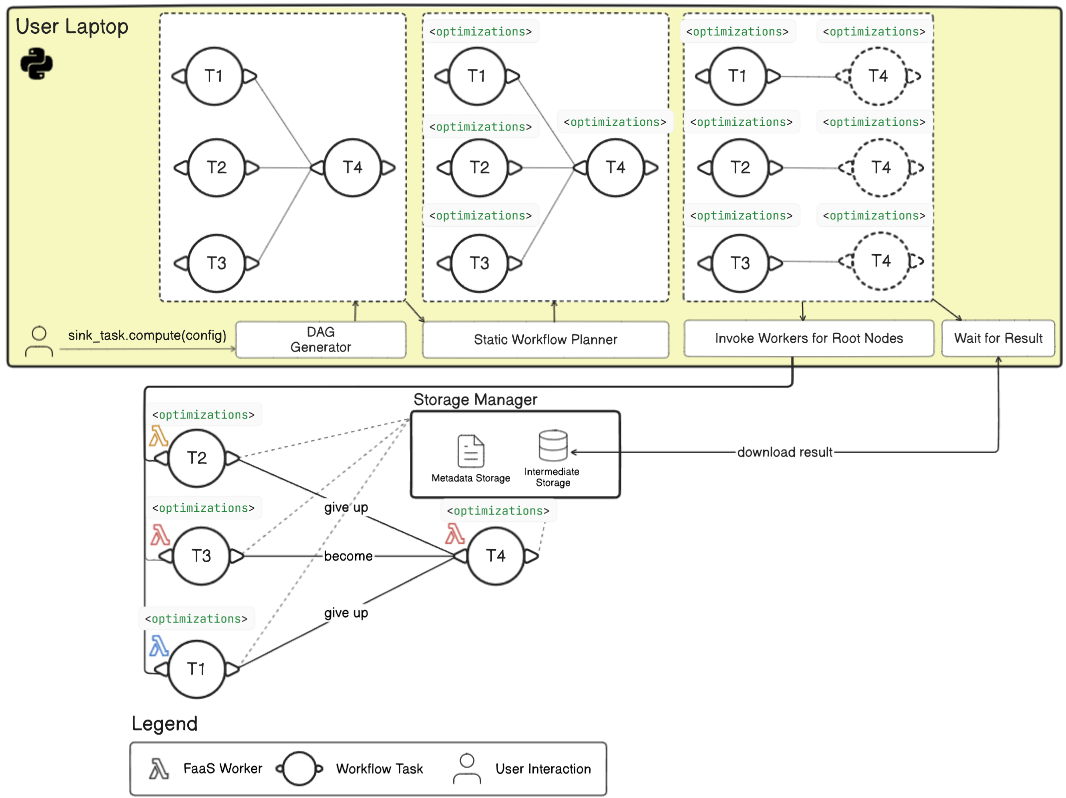
\includegraphics[width=\columnwidth]{figures/solution_distributedarchintegrated.png}
  \caption{Solution Architecture}
  \label{fig:solution_architecture}
\end{figure}

\begin{enumerate}
    \item \textbf{Metadata Management}: Responsible for collecting and storing task metadata from previous executions. It also uses this metadata to provide predictions regarding task execution times, data transfer times, task output sizes, and worker startup times;
    \item \textbf{Static Workflow Planning}: Receives the entire workflow, represented as a Directed Acyclic Graph (DAG), and a "planner" (an algorithm chosen by the user). This planner will use the predictions provided by Metadata Management to create a static plan/schedule to be followed by the workers;
    \item \textbf{Scheduling}: This component is integrated into the workers, and it is responsible for executing the plan generated by the Static Workflow Planning layer, applying optimizations and delegating tasks as needed.
\end{enumerate}

There are 3 distinct computational entities involved in this system:

\begin{itemize}
    \item \textbf{User Computer}: Responsible for creating workflow plans, submitting them (triggering workflow execution), and receiving its results. The planning phase also happens on this computer, right before a workflow is submitted for execution;
    \item \textbf{Workers}: These are the FaaS workers (often running in containerized environments), that execute one or more tasks. The decentralization of our solution is due to the fact that these workers are responsible for scheduling of subsequent tasks, delegating tasks and launching new workers when needed without requiring a central scheduler. Lastly, they are also responsible for collecting and uploading metadata;
    \item \textbf{Storage}: Consists of an \textit{Intermediate Storage} for intermediate outputs which may be needed for subsequent tasks and a \textit{Metadata Storage} for information crucial to workflow execution (e.g., notifications about task readiness and completion).
\end{itemize}

Next, we will explain how the user defines and submits workflows for execution.

\subsection{Workflow Definition Language}

The user can create workflows by composing individual Python functions, as shown in listing \ref{lst:dag_lang_example}. Here, we define two tasks, \texttt{task\_a} and \texttt{task\_b}, and then compose them into a DAG/Workflow by passing their results as arguments to the next task. The resulting workflow can be visualized in figure \ref{fig:dag_example}.

\begin{figure}[h]
\centering
\begin{lstlisting}[language=Python, basicstyle=\ttfamily\footnotesize, columns=fullflexible, breaklines=true]
# 1) Task definition
@DAGTask
def task_a(a: int) -> int:
    # ... user code logic ...
    return a + 1

@DAGTask(forced_optimizations=[PreLoadOptimization()])
def task_b(*args: int) -> int:
    # ... user code logic ...
    return sum(args)

# 2) Task composition (DAG/Workflow)
a1 = task_a(10)
a2 = task_a(a1)
a3 = task_a(a1)
b1 = task_b(a2, a3)
a4 = task_a(b1)
\end{lstlisting}
\caption{DAG definition example}
\label{lst:dag_lang_example}
\end{figure}

\begin{figure}[h]
    \centering
    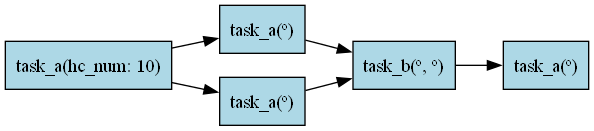
\includegraphics[width=\columnwidth]{figures/dag_lang_example.png}
    \caption{Simple DAG example}
    \label{fig:dag_example}
\end{figure}

When \texttt{task\_a(10)} is invoked, it doesn't actually run the user code. It instead creates a representation of the task, which can be passed as argument to other tasks. The workflow planning and execution only happens once \texttt{.compute()} is called on the last/sink task (\texttt{a4}), as shown in listing \ref{lst:triggering_workflow_execution}. When \texttt{compute()} is called, we can create a representation of the entire workflow structure by backtracking the task dependencies.

\begin{figure}[h]
\centering
\begin{lstlisting}[language=Python, basicstyle=\ttfamily\footnotesize, columns=fullflexible, breaklines=true]
result = a4.compute(
    dag_name="simpledag", 
    config=Worker.Config(
        faas_gateway_address=...,
        intermediate_storage_config=(ip, port, password),
        metrics_storage_config=(ip, port, password),
        planner_config=SimplePlannerAlgorithm.Config(
            sla=sla,
            worker_resource_configuration=TaskWorkerResourceConfiguration(cpus=3, memory_mb=512),
        )
    )
)
\end{lstlisting}
\caption{Triggering workflow execution}
\label{lst:triggering_workflow_execution}
\end{figure}

One limitation of this DAG definition language is that it doesn't support "dynamic fan-outs" (e.g., creating a variable number of tasks depending on the result of another task). 

We will now go into more detail about each of the 3 layers, unfolding its components and importance to the overall system.

\subsection{Metadata Management}
\label{ss:metadata_management}
The goal of the \textbf{Metadata Management} layer is to provide the most accurate task-wise predictions to help the planner algorithm chosen by the user to make better decisions. To achieve this, while the workflow is running we collect metrics about each task's execution. These metrics are stored in \textit{Metadata Storage}: task execution time, data transfer size and time, task input and output sizes, and worker startup time. 

Storing these metrics enables us to provide a prediction API, shown in Listing~\ref{lst:task_predictions_api}. To improve accuracy, metrics are kept separate for each workflow. As a result, even if two workflows use the same function or task code, their metrics are stored independently. This design choice reflects our assumption that different workflows may follow different execution patterns. To avoid introducing runtime overhead, metrics are batched and uploaded when the worker shuts down.

The prediction methods take an additional parameter, \texttt{SLA} (Service-level Agreement), which is specified by the user and influences the selection of prediction samples. For example, \texttt{SLA="median"} will use the median of the historical samples, whereas \texttt{SLA=Percentile(80)} will return a more conservative estimate. By allowing the user to control this parameter, the API can provide predictions that are tailored to different performance requirements.

\begin{figure}[h]
\centering
\begin{lstlisting}[basicstyle=\ttfamily\footnotesize, columns=fullflexible, breaklines=true]
class PredictionsProvider:
  def predict_output_size(function_name, input_size, sla) -> int
  def predict_worker_startup_time(resource_config, state: 'cold' | 'warm', sla) -> float
  def predict_data_transfer_time(
        type: 'upload' | 'download',
        data_size_bytes,
        resource_config,
        sla,
        scaling_exponent
    ) -> float
  def predict_execution_time(
        task_name,
        input_size,
        resource_config,
        sla: SLA,
        size_scaling_factor
    ) -> float
\end{lstlisting}
\caption{Task Predictions API}
\label{lst:task_predictions_api}
\end{figure}

In addition, metrics such as worker startup time, data transfer time, and task execution time are tied to the specific worker resource configuration. To account for this, our prediction method follows two paths. If we have enough historical samples for the same resource configuration, we use only those. Otherwise, when there are not enough samples with the same resource configuration, we fall back to a normalization strategy: we adjust samples from other memory configurations to a baseline, use those to estimate execution time, and then rescale the result back to the target configuration. After selecting all relevant samples we use an algorithm that selects a limited number of the most relevant samples for each prediction.

\subsection{Static Workflow Planning}
This layer executes on the user side, and it receives the workflow representation and a workflow planning algorithm chosen by the user (as shown in listing \ref{lst:triggering_workflow_execution}). Its job is to execute the planning algorithm, providing it access to the predictions exposed by the Metadata Management layer (section \ref{ss:metadata_management}).

Planners can run \textit{workflow simulations} based on the predictions, allowing them to experiment with different resource configurations for different tasks, different task co-location strategies, and different optimizations. The accuracy of this simulation depends on the accuracy of the predictions exposed by the \textit{Predictions API}.

For each task, the planner assigns both a \texttt{worker\_id} and a resource configuration (vCPUs and memory). The \texttt{worker\_id} specifies the worker instance that must execute the task—analogous to the “colors” in Palette Load Balancing~\cite{palette_load_balancing}, but in our case this assignment is mandatory rather than advisory, giving strict control over execution locality. If \texttt{worker\_id} is not specified, workers will, at run-time, have to decide whether to execute or delegate those tasks, similar to WUKONG's ~\cite{wukong_2} scheduling. We refer to these workers as \textit{"flexible workers"}.

Users can select from a 3 provided algorithms or implement their own planner by implementing an interface. All planners have access to the predictions API as well as the workflow simulation. The basic planners the user can choose from are the following:

\begin{enumerate}
    \item \textbf{Simple}: All tasks will use the same worker configuration (specified by the user) and be executed by \textit{"Flexible workers"}. This is a more dynamic scheduling approach where tasks aren't tied to specific workers;
    \item \textbf{Uniform}: All tasks will use the same worker configuration (specified by the user). Fixed worker IDs are assigned to tasks. Applies \texttt{task-dup} optimization to suitable tasks and simulates the potential benefits of using \texttt{pre-load} optimizations on tasks that are on the critical path;
    \item \textbf{Non-Uniform}: All tasks will use different worker configurations (list of available resources is specified by the user). Fixed worker IDs are assigned to tasks. This algorithm starts by assigning the best available resources to all tasks. Then it runs a resource downgrading algorithm that attempts to downgrade resources of workers outside the critical path as much as possible without introducing a new critical path. Then, similarly to the Uniform planner, it applies \texttt{task-dup} optimization to suitable tasks and simulates the potential benefits of using \texttt{pre-load} optimizations on tasks that are on the critical path. It also applies \texttt{pre-warm} optimizations to suitable tasks.
\end{enumerate}

Planners can use different optimizations to achieve their goals, whether it's extracting maximum performance or minimizing resource utilization. Similarly to planners, users can also create new optimizations and define how workers should react to them. The provided optimizations are \textbf{pre-warm}, \textbf{pre-load} and \textbf{task-dup}.

\textbf{pre-warm}(worker\_config):
\begin{itemize}
  \item \textit{Interpretation}: Tasks/Nodes with this optimization should perform a special invocation to the FaaS gateway that forces it to launch a new worker with the specified resource configuration \texttt{worker\_config}. This can be used to warm up workers ahead of time and mask cold start latencies;
  \item \textit{Assignment Logic}: For the nodes whose workers are expected to have cold starts, find the "optimal" node to perform the pre-warming by searching for nodes/tasks whose activity timing falls within a window (goal: avoid the pre-warmed worker from going cold before needed, while also not being warm too late). The optimization will be added to the "optimal" node, which will be responsible for doing the special "empty invocation" to the FaaS gateway.
\end{itemize}

\textbf{pre-load}:
\begin{itemize}
  \item \textit{Interpretation}: Workers assigned to tasks or nodes with this optimization should begin downloading the task's dependencies as early as possible. This prevents scenarios where a worker must fetch all dependencies at once. The optimization is effective only if the worker is active before executing the task, allowing it to download dependencies in parallel with other ongoing tasks. This is implemented by having the worker receive completion notifications from the \textit{Metadata Storage} for all tasks upstream of the optimized task;
  \item \textit{Assignment Logic}: This is an iterative process that optimizes the workflow along its critical path. First, the algorithm identifies the critical path and assigns the optimization to eligible nodes on it. The critical path is then recalculated: if the total execution time increases, the optimization is removed; if the execution time decreases but the critical path changes, the algorithm restarts with the new path. This process repeats until no further improvements are possible, or the algorithm hits a fixed iteration limit.
\end{itemize}

\textbf{task-dup} [Task Duplication]:
\begin{itemize}
  \item \textit{Interpretation}: Tasks or nodes with this optimization can be executed by other workers if doing so helps unlock dependent tasks more quickly. The task could be "duplicated" by workers that depend on its output. It is a trade-off between performance and resource utilization, allowing potentially faster execution at the cost of using additional compute resources;
  \item \textit{Assignment Logic}: Assigned to all nodes whose execution time and input size do not exceed predefined thresholds. Whether duplication actually occurs is decided at run-time. The optimization targets fast tasks with small inputs, as these are inexpensive to duplicate in terms of both downloading dependencies and execution. This way, even if duplication turns out to be unnecessary, the impact on performance and resource usage remains minimal.
\end{itemize}

For simplicity, all planners currently use the same optimization assignment logic, so both \textit{Uniform} and \textit{Non-Uniform} planners apply identical criteria when assigning optimizations to tasks. However, this is not a strict requirement—different planners could adopt their own assignment strategies.

Because planners may sometimes lack sufficient information to make optimal decisions about optimization assignments, it is important to allow users to specify optimizations for specific tasks manually. An example of this feature is shown in Listing~\ref{lst:dag_lang_example}, where the user requests that \texttt{task\_b} attempt to \textit{pre-load} its dependencies.

Once these optimizations are assigned, workflow planning is complete, and workers can begin execution. Because planning occurs on the user's machine, it is responsible for initiating the workflow by starting the initial workers. From that point onward, workers dynamically invoke additional workers as needed, following a choreographed, decentralized execution model.

\subsection{Scheduling}

%TODO: explain what are the workers: FaaS workers
%TODO: when they are started, they fetch the DAG from Metadata Storage
%TODO: they emit and listen for TASK_READY and TASK_COMPLETED events to make optimizations possible
%TODO: they use a dependency counter (similar to WUKONG) atomic integer to detect when a task is ready

% ------------------------------------------------ %

\section{Evaluation and Analysis}

\subsection{Testing Environment}
%TODO: explain Docker simulating faas environment
\subsection{Testing Configurations}
%TODO: worker resources, workflows, planners, SLAs

\section{Conclusion}

\bibliographystyle{IEEEtran}
\bibliography{references}

\end{document}
